%%This is a very basic article template.
%%There is just one section and two subsections.
\documentclass[12pt]{jreport} 
%\usepackage{kmd-emthesis} %English
\usepackage{kmd-jmthesis}
\usepackage{graphicx}
%\usepackage{subfigure}
\usepackage{tabularx}
\usepackage{longtable}
\usepackage{multirow}
\usepackage{url}
\usepackage{fancybox}
\usepackage{amssymb}
\usepackage{moreverb}
\usepackage{afterpage}
\usepackage{cite}
%\usepackage{harvard-oikos}
\usepackage{ccaption}     % caption操作
\usepackage{fn2end} %脚注を文末注に一斉変更するパッケージ
\usepackage{fn2end_config} %脚注にインデントをつけるパッケージ
\usepackage{color}
%%%%%%%%%%%%%%%%%%%%%%%%%%%%

\makeatother
%
%
% ページスタイルの指定
\pagestyle{final}       % 清書
%\pagestyle{draft}      % 下書き
%
% 使用言語の指定
\lang{Japanese} % 日本語
%\lang{English} % 英語
%
% 学生番号
\studentnumber{81335042}
%
% 修士論文 か 課題研究 かの選択
\doctitle{\mastersthesis}       % 修士論文
%\doctitle{\mastersreport}      % 課題研究
%
% 取得予定の修士号
\major{\mediadesign}    % メディアデザイン学
%
% 日本語題目 (in LaTeX)
\title{レクリエーション分野における\\フラッシュマーケティングの活用}
%
% 日本語題目 (in plain text)
%   注: (in LaTeX)と同じ場合は指定する必要なし。
%       この情報は修士論文/課題研究には現れませんが、管理のために必要です。
\ptitle{レクリエーション分野における\\フラッシュマーケティングの活用}
%
%
% 英語題目 (in LaTeX)
\etitle{Practice of Design Thinking Workshop to Develop\\ ``Media Innovator'' Leading Creative Society}
%
% 英語題目 (in plain text)
%   注: (in LaTeX)と同じ場合は指定する必要なし。
%       この情報は修士論文/課題研究には現れませんが、管理のために必要です。
\eptitle{Practice of Design Thinking Workshop to Develop ``Media Innovator'' Leading Creative Society}%
%
% 日本語氏名 (in LaTeX)
%   (姓と名の間に空白を入れて下さい)
%
\author{飯田 光}
%
% 日本語氏名 (in plain text)
%
%   注: (in LaTeX)と同じ場合は指定する必要なし。
%       この情報は修士論文/課題研究には現れませんが、管理のために必要です。
%
\pauthor{飯田 光}
%
% 欧文氏名 (in LaTeX)
%   (first name, last name の順に記入し、先頭文字のみを大文字にする。)
%
\eauthor{Hikaru Iida}
% 別の例: \eauthor{Kurt G\"{o}del}
%
%
% 欧文氏名 (in plain text)
%
%   注: (in LaTeX)と同じ場合は指定する必要なし。
%       この情報は修士論文/課題研究には現れませんが、管理のために必要です。
%
\epauthor{Hikaru Iida}
% 別の例: \peauthor{Kurt Goedel}
%
%

% 論文提出年度(Academic Year)
\syear{2014}
\heiseiyear{26}
%\smonth{2}
%\sday{7}

%
%
% 指導教員(日本語)
%   (姓と名、名と称号の間に空白を入れて下さい)
%
\chmembers{杉浦 一徳 教授}{(主指導教員)}
         {岸 博幸 教授}{(副指導教員)}
         
%
%
% 審査委員(日本語)
%   (姓と名、名と称号の間に空白を入れて下さい)
%
%5人の場合、5人目は\addcomembers を使って宣言する
%主指導教員、副指導教員を明記する。両指導教員以外は委員。
%\comembers{砂原 秀樹 教授}{(主指導教員)}
%         {加藤 朗 教授}{(副指導教員)}
%         {河口 信夫 教授}{(委員、名古屋大学)}
%         {○○ ○○ 准教授}{(委員)}
%
%\addcomembers{×× ×× 助教}{(委員)}
%4人の場合
%\comembers{砂原 秀樹 教授}{(主指導教員)}
%         {加藤 朗 教授}{(副指導教員)}
%         {河口 信夫 教授}{(委員、名古屋大学)}
%         {○○ ○○ 准教授}{(委員)}
% 3人の場合
\comembers{杉浦 一徳教授}{(主査)}
         {岸 博幸 教授}{(副査)}
         {稲見 昌彦 教授}{(副査)}
         {}{}
\addcomembers{}{}
% 2人の場合
%\comembers{砂原 秀樹 教授}{(主指導教員)}
%         {加藤 朗 教授}{(副指導教員)}
%
% 指導教員(英語)
%     (first name, last name の順に記入し、先頭文字のみを大文字にする。
%       first name と last name の間に空白、
%       last name と 称号の間にカンマと空白を入れて下さい。)
\echmembers{Professor kazunori Sugiura}{(Supervisor)}
          {Professor Hiroyuki Kishi}{(Co-supervisor)}
% 審査委員(英語)
%     (first name, last name の順に記入し、先頭文字のみを大文字にする。
%       first name と last name の間に空白、
%       last name と 称号の間にカンマと空白を入れて下さい。)
%
% 5人の場合、5人目は\eaddcomembers を使って宣言する
% Supervisor, Co-supervisor, and Member must be specified.
%\ecomembers{Professor Shunsuke Uemura}{(Supervisor)}
%          {Professor Minoru Ito}{(Co-supervisor)}
%          {Associate Professor Masatoshi Yoshikawa}{(Member, Nagoya University)}
%          {Associate Professor xxxxxx xxxxxx}{(Member)}
%\eaddcomembers{Associate Professor oooooo oooooo}{(Member)}
% 4人の場合
%\ecomembers{Professor Hideki Sunahara}{(Supervisor)}
%          {Professor Akira Kato}{(Co-supervisor)}
%          {Professor Nobuo Kawaguchi}{(Member, Nagoya University)}
%          {Associate Professor xxxxxx xxxxxx}{(Member)}
% 3人の場合
\ecomembers{Professor Kazunori Sugiura}{(Supervisor)}
          {Professor Hiroyuki Kishi}{(Co-supervisor)}
          {Associate Professor Kazunori Sugiura}{(Member)}
          {}{}
\eaddcomembers{}{}
% \ecomembers{Professor Hideki Sunahara}{(Supervisor)}
%           {Professor Akira Kato}{(Co-supervisor)}
%           {Professor Nobuo Kawaguchi}{(Member, Nagoya University)}
% 2人の場合
% \ecomembers{Professor Hideki Sunahara}{(Supervisor)}
%           {Professor Akira Kato}{(Co-supervisor)}
%
% キーワード5個 (in LaTeX)
%
\keywords{フラッシュマーケティング、消費者行動、共同購入、ギャザリング、O2O}
%
% キーワード5個 (in plain text)
%
%   注: (in LaTeX)と同じ場合は記入する必要なし。
%       この情報は修士論文/課題研究には現れませんが、管理のために必要です。
%
\pkeywords{フラッシュマーケティング、消費者行動、共同購入、ギャザリング、O2O}
%
% 5 or 6 Keywords (in LaTeX)
%
\ekeywords{Flash Marketing, Consumer Behavior, group-buying, Gathering, O2O}
%
% 5 or 6 Keywords (in plain text)
%
%   注: (in LaTeX)と同じ場合は記入する必要なし。
%       この情報は修士論文/課題研究には現れませんが、管理のために必要です。
%
\epkeywords{Design Thinking, Creative Society, Workshop, Innovation, Education}

%論文の投稿カテゴリーを一つ選ぶ(デザイン, サイエンス / エンジニアリング, アクションリサーチ, 社会科学 / 人文科学)
\category{アクションリサーチ}
%論文の投稿カテゴリーを一つ選ぶ(デザイン, サイエンス / エンジニアリング, アクションリサーチ, 社会科学 / 人文科学)(in plain text)
\pcategory{アクションリサーチ}

%Choose one submission category from [Design, Science / Engineering, Social Science / Humanities, Action Research]
\ecategory{Action Research}
%Choose one submission category from [Design, Science / Engineering, Social Science / Humanities, Action Research] (in plain text)
\ecategory{Action Research}


%
% 内容梗概 (in LaTeX)
%
%   注: 行の先頭が\\で始まらないようにすること。
%
\abstract{
近年、フラッシュマーケティング(以下、FM)という手法を用いて、ビジネスを展開する企業が増えてる。フラッシュマーケティングとは、商品やサービスの提供にあたり、割引価格や特典がついたクーポンを期間限定でインターネット上で販売する手法である。一般に24時間から72時間程度の短時間(フラッシュ)に、集客と販売および見込み顧客の情報収集が行われるという特徴を持つ。米国では従来から販売期間を24時間と短く設定した "One deal a Day" ("Deal of the day")という手法が存在しており、Amazon.comやBuy.comが採用していた。2008年GROUPON社が、割引クーポンをインターネット上で事前に共同購入するビジネスモデルを始める。このメソッドは、GROUPON社の海外進出に伴い世界に広まり、類似サービスも出現していく。
日本市場においても、FMを用いたビジネス領域が拡大するものの、特定の領域に偏って発展している傾向がある。特に、レジャーカテゴリー領域への売上が極端に低い。本研究執筆に先立ち、調査を行ったところチーム間のマッチングという付加価値が必要であることがわかり販売対象が広がりFM市場全体の売上貢献につながると考えた。
本論文は、GROUPONなどが代表に挙げられる共同購入型FMサイトに、マッチング機能を加えたフットサルコートの共同購入型マッチングサービスを提案したものである。本サービスは、チーム人数が少ないフットサルチームを対象に格安でフットサルコートを提供する一方で、コート運営者側はアイドリングの時間を削減することができる
本論文では、FMサイトにおけるビジネスモデルの変化、現在のレジャー施設、ユーザーにFMサイトの意識調査を行い、FMサイトの実態と照らし合わせた。その結果、購入する際のユーザー側の問題、フットサルコート側の集金リスクが課題であることが分かった。この問題を解決するために、FMサイトでユーザー間のマッチングを図り、当サイトがフットサルコートの代わりに集金を担い実証実験を行った。
従来のフットサルチーム同士が交流する大会のように、審判やタイムキーパーがいなければチーム間での試合は成立しないと考えられてきたが、事前に大会チュートリアルメールを送ることと前払い制度を導入することで、試合の運営に関する上記のボトルネックは解消された。またフットサルコートは空き時間を有効に活用することができ、会員登録制の施設を要するスポーツジャンルであれば展開できる可能性を示した




}
% Abstract (in plain text)
%
%   注: (in LaTeX)と同じ場合は記入する必要なし。
%       この情報は修士論文/課題研究には現れませんが、管理のために必要です。
%       改行する箇所には空白行を入れる。
%       行の先頭が\\で始まらないようにすること。
%
\eabstract{
The Graduate School of Media Design (KMD) was established to train talented individuals to work on the global stage building and running new industries for the coming ``creative society,'' a world in which the driving force of the economy will be creativity rather than productivity or efficiency. ``Creativity'' is the ability to produce new ideas, expressions, and processes. These new creations and the activities inspire give rise to an economic base with the power and energy to bring forth innovative technologies and enrich human societies. The work of the individual is paramount in the creative society; consumers lead creative activities. Collaboration is all-important. Individuals innovate, mutually recognizing a diversity of values and making personal, imaginative contributions that collectively result in extraordinary achievements and capacities.
}
%%%%%%%%%%%%%%%%%%%%%%%%% document starts here %%%%%%%%%%%%%%%%%%%%%%%%%%%%


\begin{document}
%
% 表紙 および アブストラクト
%
\titlepage
\comemberspage
\firstabstract
\secondabstract
%
% 目次
%
\toc
\newpage
\listoffigures
\newpage
\listoftables
%
% これ以降本文
%
\newpage
\pagenumbering{arabic}
\chapter{序論}
\label{intro}
\section{背景}
近年、フラッシュマーケティングという手法を用いて、ビジネスを展開する企業が増えてる。フラッシュマーケティングとは、商品やサービスの提供にあたり、割引価格や特典がついたクーポンを期間限定でインターネット上で販売する手法である。一般に24時間から72時間程度の短時間に、集客と販売および見込み顧客の情報収集が行われるという特徴を持つ。ふた。米国では従来から販売期間を24時間と短く設定した "One deal a Day" ("Deal of the day")という手法が存在している。2008年GROUPON社が、割引クーポンをインターネット上で事前に共同購入するビジネスモデルを始める。このメソッドは、GROUPON社の海外進出に伴い世界に広まり、類似サービスも出現していく。
日本市場においても、フラッシュマーケティングを用いたビジネス領域が拡大するものの、特定の領域に偏って発展している傾向がある。特に、レジャーカテゴリーへの売上が極端に低い。このカテゴリー内でフットサルコートのコート数は年々伸びているが、十分にコートへ送客できているとは言えない。本研究執筆に先立ち、調査を行ったところチーム間のマッチングという付加価値が必要であることがわかり販売対象が広がりフラッシュマーケティング市場全体の売上貢献につながると考えた。

\subsection{レクリエーション市場における市場推移}

\subsection{フットサル市場の推移}
次にフットサルの市場推移をコート数と参加人数の推移を基に見ていく。まずフットサルコートは年々増加傾向にあり、特に2002年のサッカー日韓ワールドカップを機に首都圏を中心に増加した。ワールドカップの盛り上がりを背景に、少人数で手軽にサッカーに近い競技を楽しめることがコートの増加に拍車をかけた。



\begin{figure}[htbp]
	\centering
	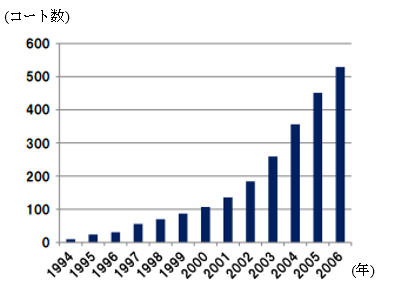
\includegraphics[width=85mm, bb=0 0 330 272]{figures/court.jpg}
	\caption{データ引用元 {\itshape レジャー白書2007}}
	\label{レジャー白書2007}
\end{figure}

フットサルプレイヤーの数はやや鈍化傾向にあるが、未だに緩やかな右肩上がりの成長を続けていると言える。
現在では、フットサルのプロリーグであるFリーグをはじめ、全国リーグ、公式戦・地方トーナメント・芸能人リーグの開催と共に、着実に競技人口を増やしつつある。

\begin{figure}[htbp]
	\centering
	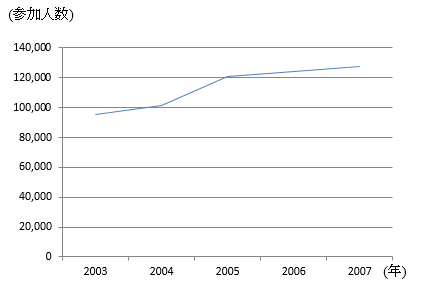
\includegraphics[width=85mm, bb=0 0 330 272]{figures/pati.jpg}
	\caption{データ引用元 {\itshape www.salon20002.net/monthly/2008/2008-22.pdf}}
	\label{www.salon20002.net/monthly/2008/2008-22.pdf}
\end{figure}

このように年々、フットサルコートは増えているが、フットサルプレイヤーの数は増えていない。特に東京郊外のフットサルコートのレンタルだけでは、運営が難しいので、フットサルスクールや大会を開催し、運営しているコートが多々ある。

\section{フラッシュマーケティングを用いた集客の取り組み}
次の章で詳細を述べるが、フラッシュマーケティング市場においてレクリエーションカテゴリが占める売上の割合は10%程であり、特にフットサルコートを始め、会員制クラブでもフラッシュマーケティングサイトが占める割合は少ない。ここでは、フットサルコートでフラッシュマーケティングが適用された事例を見ていく。

\subsection{LaBOLAクーポン}
 株式会社ラクシーズは2010年12月6日より、スポーツ・レジャーに特化した事前購入型クーポンサービス「LaBOLAクーポン」を開始し、フラッシュマーケティングに参入した。
LaBOLAクーポンとは、スポーツ・レジャーに特化したプレミアムクーポンを購入できるサービスであり、フットサルおよびサッカー情報提供サービスサイトを運営するラクシーズが運営しているスポーツSNS「LaBOLA(ラボーラ)」との連携による相乗効果を狙った。LaBOLAの会員数は2010年当時約10万人超。月間アクセス数 約300万PV。ユニークユーザー数は約50万人に及んでおり、既に会員を有しているコミュニティーとの連携は大きなアドバンテージと考えられていた。
\\ しかし2011年9月30日をもってサービスは終了している。元々フットサル、サッカーに特化したSNSのLaBOLAの顧客に対し、ヨガやゴルフ教室といったクーポンを提供していたことが、既存の顧客に対しての興味関心の相違がサービスの売上が伸び悩んだことの要因と考えられる。
\newpage

\subsection{Grouponにおけるレジャー施設の活用方法}
2010年から日本国内でサービスを始めたGrouponは、フットサルコートのクーポンの販売もしている。2012年まではコートのクーポンを販売していたが、近年では図にあるようにコートの使用だけではなく有名人をと一緒にフットサルを楽しめるイベント型のクーポンも販売している。都内のフットサルコートでは、イベント型のクーポンが増えている。
\\ 次の小節で詳しくフットサルコートがフラッシュマーケティングを取り入れない理由を述べるが、このようにクーポン自体に使用以外に他の特典を付けた理由は、フットサルコートのオーナーの調査を行った結果、以下二点が考えられる。
\\・利用者がクーポン購入後の使い方がよくわからない
\\・空きコートを掲載できるのが一日だけなので、購入されなえればそのまま空きコートのなる可能性が高い
\\
\\
\\
\\
\\
\\
\\
\begin{figure}[htbp]
	\centering
	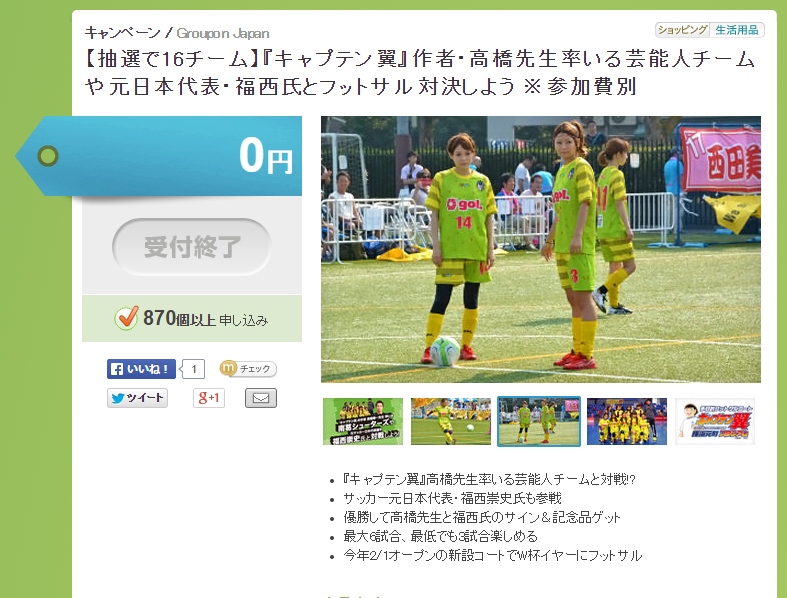
\includegraphics[width=85mm, bb=0 0 400 272]{figures/cap.jpg}
	\caption{データ引用元 {\itshape http://www.groupon.jp/cid/103608}}
	\label{www.salon20002.net/monthly/2008/2008-22.pdf}
\end{figure}


\section{問題提起}
上記のように、レクリエーション分野、特にフットサルコートにおいて、フラッシュマーケティングは上手く活用できているとは言えない。
そこで筆者は八王子、多摩地区所在する5つのフットサルコートのオーナーと首都圏を中心にフットサルコートを運営するエリアマネージャーにインタビュー調査を行い、フラッシュマーケティングの問題点とフラッシュマーケティングを用いらない理由を調査した。

\begin{itemize}
	\item 利用者がクーポン購入後の使い方がよくわからない
	\item 空きコートを掲載しても、購入されなえればそのまま空きコートのなる可能性が高い
	\item クーポンを出稿する際の文言を考えたり、手間がかかること。
	\item そもそもフラッシュマーケティングサイトに出稿されていることをフットサルプレイヤーはしらない
	\item ターゲット対象が、ある程度練習頻度が多いチームでないといけない
	\item そもそもクーポン購入客専用の対応を作らなければいけない
\end{itemize}



チーム人数が少ないフットサルチーム複数に対して、格安でフットサルコートを提供することで、コート運営者側はアイドリングの時間を削減することができ下記の問題を解決できると考えた。
\\・チーム人数の少ないチームはクーポンを買うことができない
\\・マッチング後の試合の運営方法
\\・コートの価格が高すぎる
\\・コートの集金リスクを軽減する

\section{実証と検証}
フラッシュマーケティングサイトにおけるビジネスモデルの変化、現在のレジャー施設、ユーザーにフラッシュマーケティングサイトの意識調査を行い、フラッシュマーケティングサイトの実態と照らし合わせた。その結果、購入する際のユーザー側の問題、フットサルコート側の集金リスクが課題であることが分かった。この問題を解決するために、フラッシュマーケティングサイトを構築し、ユーザー間のマッチングを図り、当サイトがフットサルコートの代わりに集金を担い実証実験を行った。
\section{本論の構成}
%\makeendnotes  %フットノートをすべて章末に移動するスクリプトです。使用しない場合はコメントアウトしてください。
本論の構成はまず1章で現状のレジャー施設の現状分析を行った後に、2章でフラッシュマーケティングに関する先行研究を述べ、本サービスに必要部分を抽出する。3章ではプロトタイプを用いり、ユーザーテストを行った。4章ではユーザーテスト時のユーザーのコメントを基に、サービスコンセプトを決めた。プロトタイプを修正したものを実際にサービスとして、各フットサルコートと提携し、運営内容を述べる。6章ではサービスの評価を行い、7章で結論を述べる。


%改ページしたい場合
%\newpage

%%%%%Notes%%%%%
%エンドノートを使用しない場合は以下をコメントアウトしてください。
\section*{注}
\addcontentsline{toc}{section}{注}
\begin{footnotesize}
%\theendnotes
\end{footnotesize}


\chapter{関連研究}
\makeendnotes  %フットノートをすべて章末に移動するスクリプトです。使用しない場合はコメントアウトしてください。

\section{フラッシュマーケティングについて}
\subsection{フラッシュマーケティングとは}
フラッシュマーケティングとはインターネットを使って、商品やサービス利用料をクーポンとして割り引き販売する手法のことである。“フラッシュが光るような短期間”で販売し終えることからちなんで名づけられた。そのため販売時間は24時間~48時間という短時間がほとんどで、この間に出品者が設定した数量が売り切れれば取引が成立し、予定数の注文に達しなければ販売は成立しないというシステムになっている。
また宣伝効果も期待でき、話題性のある商品を出品することで、SNSといった口コミを誘いやすく、宣伝効果は高い。専用サイトでは、取引成立までの残時間をカウントダウン表示することで、購買意欲を高めるなどの工夫があるのが特徴だ。

具体的に従来のクーポンサイトとの違いは矢内で以下5つが挙げられている。
\begin{enumerate}
	\item \textbf{消費の前にチケットを購入する必要がある}
	\\事前購入という方法は、消費者にとっては負担が大きいが、店舗の視点から考えれば売り上げが見込め、従来の街角で配布しているクーポンに比べ、広告費の削減につながる。
	\item \textbf{購入のための期間が限定されている}
	\\期間が限定されていることで、消費者の注目を集める大きな要素となっており、消費者の決断を迫るリアクタンス理論 (Brehm, 1966; Brehm  Brehm,1981) を用いた効率的な販売手法である。
	\item\textbf{取引成立の最少人数が決まっている}
	\\最少人数を設定することで、人数に達しなければ成立しないので、成立させたいという思いから友人や他社をSNS等々でクーポンの情報を拡散させる。実際に2012年8月21日~9月20日の31日間に行われた398件の取引の分析結果を見ると10件しか不成立に終わっていない \cite{yauchi}
	また米国GROUPONの購読者調査によると66%がGROUPONの記事を見ている。結果として魅力的なクーポンが出された場合には即座に成立することになる。
	\\店舗側からすると削減される費用を割引として還元することで、他のクーポンよりも思い切った値段設定ができるという仕組みである。
	\item \textbf{割引率が高いものが多く、50%を超えるものが一般的}
	\\フラッシュマーケティングサイトの一番の特徴ともいえるのが価格の割引率である。新規開店やリニューアル、低稼働時など様々なシーンでクーポンを出して集客を図るのがフラッシュマーケティングの一般的な使い方である。
	\\先述した期間限定の特徴とも相まって消費者の意識をひきつけ購買へ結びついてると考えられる。
	\item \textbf{特定の業種に限った紹介ではなく、一般的には1day 1area 1deal 形式で様々な形式が紹介される}
	\\ぐるなびや一休のような従来のインターネット経由のクーポンの提供方法は、特定の業種に絞ってクーポンが提供されることが通例であった。これではユーザーは特定のサービスが必要な時にだけサイトに接触することになりユーザーとの接点は途切れがちになる。
	\\上記のサイトに比較してフラッシュマーケティングサイトは様々なクーポンを提供できるのだが、1day 1area 1dealという形式をとっている。これは従来のあふれんばかりの情報を整理し、消費者の居住地や趣味嗜好を基にシンプルな提案を行うことで購買活動を促している。
\end{enumerate}

\subsection{フラッシュマーケティングサイトのビジネスモデル}
上述のように、クーポン購入者を時間限定でサイト上で募集し、申し込みが規定数を超えれば割引された特別価格でのクーポンの発行が成立する。売り上げの 20〜50%は手数料として共同購入サイトに払われ、残りは店舗側の利益として支払われる。結果、クーポン購入者へは店舗側からサービスが提供される。
\\
\begin{figure}[htbp]
	\centering
	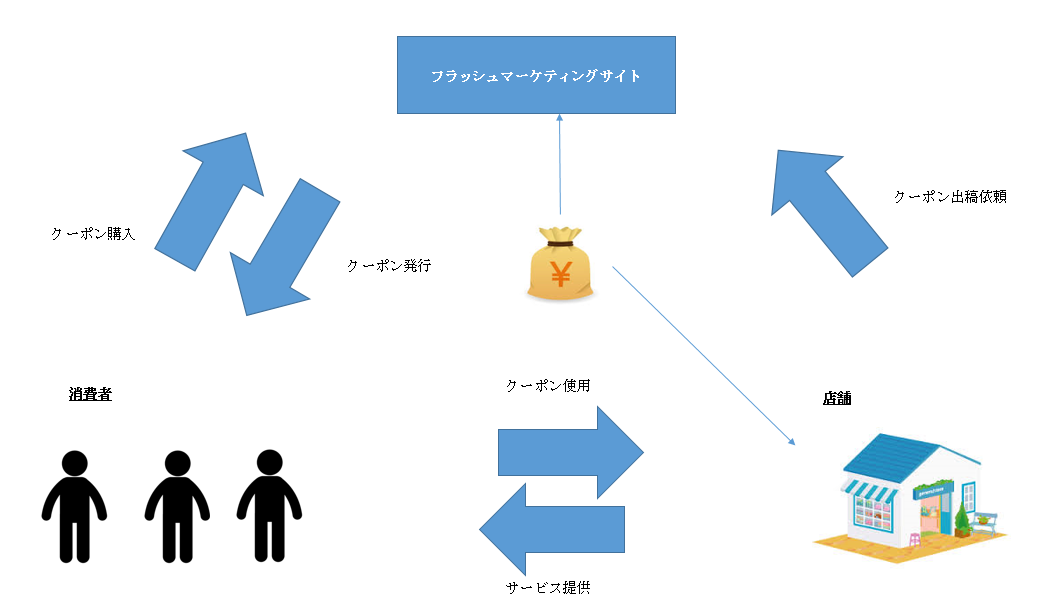
\includegraphics[width=6cm, bb=0 0 640 480]{figures/soukin.jpg}
	\caption{ビジネスモデル}
	\label{ビジネスモデル}
\end{figure}
\\
\\
店舗側からすれば客の入りが少ない時間帯を格安で提供することで、消費者を呼ぶことができ、新規顧客の獲得につながる。
\subsection{フラッシュマーケティングサイトの販売手法の転換}

次にフラッシュマーケティングの歴史について紹介する。フラッシュマーケティングの歴史は共同購入にあるといわれている。共同購入とは国内では生協のかつての販売スタイルに起因する。生協の組合員が一週間以上前に注文した商品が、翌週に班やグループに配達される仕組みのことを指す。(川口、毛利、和歌森、2005) 複数人で一つの商品を購入することで送料を下げることができ安価に購入できるというメリットがあった。1970年代にはこの無店舗事業で生協は首都圏で大きく売り上げ伸ばしていった。
\\ しかしこの生協のモデルは後に誰がどの様な商品を、購入しているのかわかってしまう、近所付き合い上やめにくくなってしまうなど人間関係上多くのデメリットがあり、人々は個人の宅に配送する宅配コープデリ (個送) を選択するようになる。
\\
\\
\begin{figure}[htbp]
	\centering
	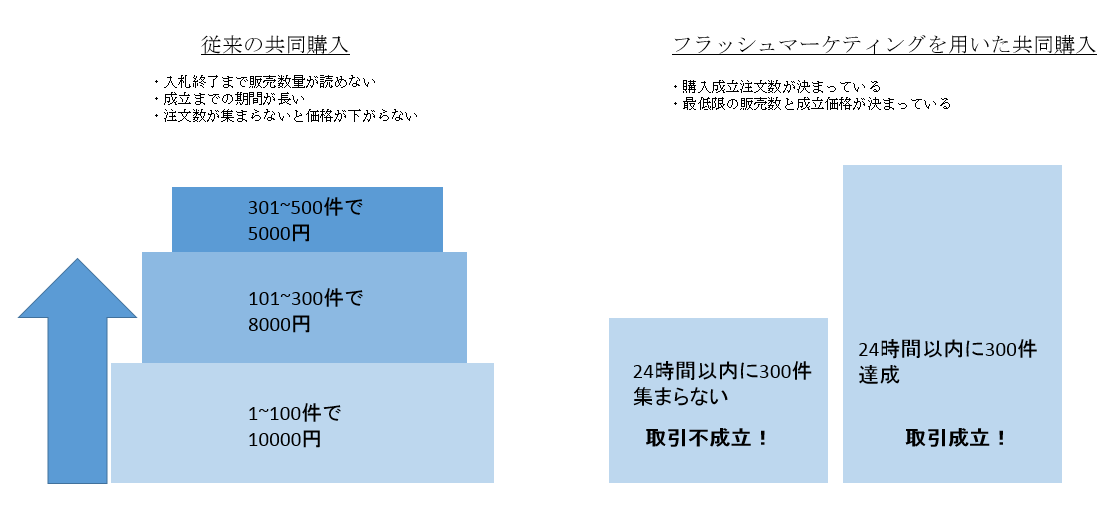
\includegraphics[width=85mm, bb=0 0 600 272]{figures/fm.jpg}
	\caption{フラッシュマーケティング市場推移 {\itshape coupon-jp.com}}
	\label{フラッシュマーケティング市場推移}
\end{figure}
\\2000年にはいるとインターネットが普及し始め、インターネット上で共同購入サイトが勃興し始めた。当初は左図のような仕組みで共同購入がの仕組みがとられていた。時間内に共同購入者を募れば募るほど、商品を割引されていくことがメリットであった。しかし以下2点の問題があった。(日経ビジネス、「話題のフラッシュマーケティングの全てがわかる」)
\begin{itemize}
	\item 注文数が集まらないと価格が下がらない
	\item 入札までの販売数がわからない
\end{itemize}

従来の共同購入では、利用者側からすると、購入した後に自身の希望する金額に減額するまでは、共同購入者を募らなければならず、最終的な購買価格もましてや購入できるのかどうかさえわからない。従来の共同購入は入札期間が1週間以上あるので、利用者は購入を先延ばしにする傾向にあり、店舗側と共同購入サイトは機会損失を生みやすかった。
\\ フラッシュマーケティングを用いり、最低成立人数を決めることで、一定の人数を集めることで、商品を購入でき、最低限の販売数も読めるようになり近年の見られるように売上が上昇した。

\subsection{フラッシュマーケティングの現状}
日本では2010年4月にサービス開始したグルーポンをはじめ、ポンパレがシェアを占めている。大手企業も参入し、リクルートのポンパレ、楽天グループのRaCoupon「買うクーポン」などがある。2010年6月時点では6社参入であったが、2010年10月時点で100サイトを超え、2011年12月時点では230サイトを超えている
日本国内におけるフラッシュマーケティングの市場推移はほぼ横ばい状態で月の売り上げは30億円程度で推移している。毎年多く企業がフラッシュマーケティング市場に参入するがグルーポンとポンパレで市場の8割ほどを占めている。
\\
\begin{figure}[htbp]
	\centering
	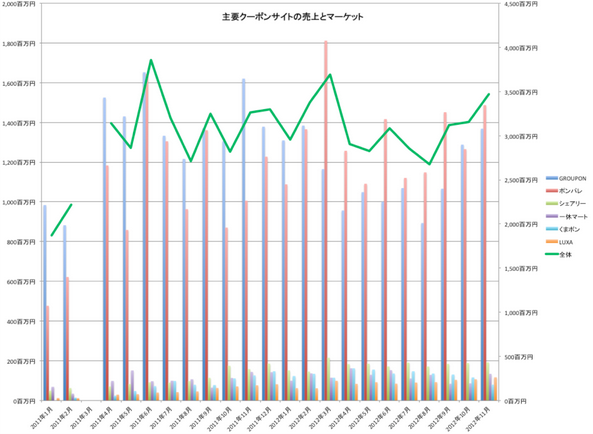
\includegraphics[width=6cm, bb=0 0 330 272]{figures/shijo.jpg}
	\caption{フラッシュマーケティング市場推移 {\itshape coupon-jp.com}}
	\label{フラッシュマーケティング市場推移}
\end{figure}
\newpage
日本国内の売上をカテゴリー別で売上を見ると、飲食の売上が圧倒的に占めている。さらに日本国内の割合とアメリカのフラッシュマーケティング市場の代替指標としてのグルーポンUS、中国のフラッシュマーケティング市場の代替指標としての中国の主要サービス10社の売上をカテゴリー別に比較した。ここでも飲食の割合が大きいのは元々、食べログやホットペッパーといった飲食におけるクーポンサイトが存在し、消費者にとって飲食分野における教育コストが低かったことが考えられる。
\begin{figure}[htbp]
	\centering
	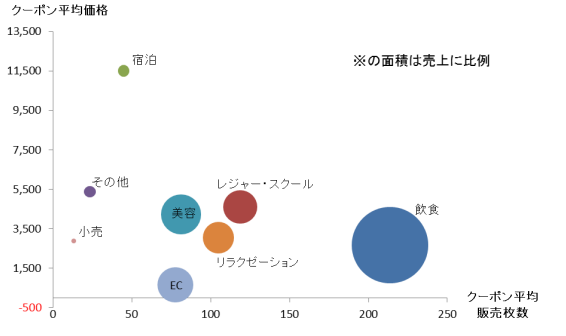
\includegraphics[width=6cm, bb=0 0 330 272]{figures/cate.jpg}
	\caption{各カテゴリー別売上 {\itshape yauchi,2012}}
	\label{各カテゴリー別売上}
\end{figure}
\begin{figure}[htbp]
	\centering
	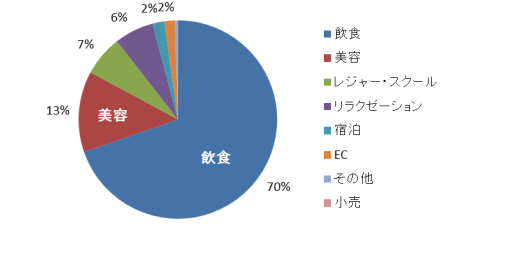
\includegraphics[width=6cm, bb=0 0 330 272]{figures/gjp.jpg}
	\caption{国内フラッシュマーケティングの売上割合 {\itshape http://ipfm.jp/dl/101224FlashMarketingFreeVER1-1.pdf}}
	\label{国内フラッシュマーケティングの売上割合}
	\end{figure}
	
\begin{figure}[htbp]
	\centering
	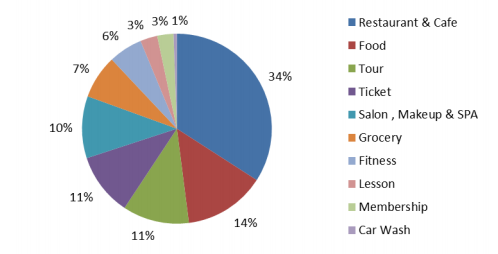
\includegraphics[width=6cm, bb=0 0 330 272]{figures/gus.jpg}
	\caption{グルーポンのアメリカにおけるカテゴリー別売上 {\itshape coupon-jp.com}}
	\label{グルーポンのアメリカにおけるカテゴリー別売上}
\end{figure}

\begin{figure}[htbp]
	\centering
	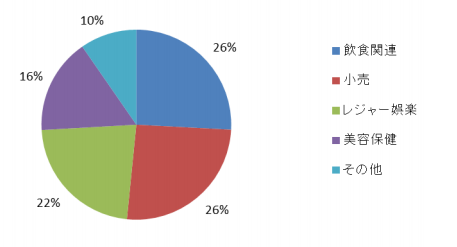
\includegraphics[width=6cm, bb=0 0 330 272]{figures/gc.jpg}
	\caption{中国におけるにおけるフラッシュマーケティング市場のカテゴリー別売上 {\itshape coupon-jp.com}}
	\label{中国におけるにおけるフラッシュマーケティング市場のカテゴリー別売上}
\end{figure}
\section{各サイトの特徴}
この節では国内の代表的なフラッシュマーケティングサイトを紹介する。
\subsection{Gropon}
Grouponは、アメリカ合衆国イリノイ州シカゴに本社を置き、共同購入型クーポンサイト「Groupon」を運営する米国の企業である。2008年10月にシカゴのピザ半額キャンペーンから始まった。日本国内では2010年6月にサービスを開始し、現在では国内の売上シェア1位である。
\\顧客獲得方法は、友人を紹介した利用者に対し、1000円程度のサイト内で使えるクーポンを配布したことで、顧客を増やしてきた。
\\国内でシェアを獲得できた理由は、従来の後払い時にクーポンを提示する従来のクーポンに対し、Grouponは前払い決済でサービスを受けられるので、クーポン発行後の損失がなく、大幅値引きが可能で利用率も高くなった。飲食、美容系(ヘアサロン、ネイルサロンなど)など後払いなので、クーポンを多数発券しても利用率は低くかったが、Grouponが前払いを採用し、利用率は上昇し、効果の見えるプロモーションが可能になったと言われている。
\subsection{ポンパレ}
ポンパレは全国に幅広い営業拠点をもつ株式会社リクルートライフスタイルが提供するフラッシュマーケティングサイトである。同業界では後発のサービスであるが、他社とは対照的にレジャー・スクールのクーポンの割合が多く、国内の市場では売上シェアが2位である。
対応エリアは東京、大阪などの主要都市から始まり、2010年11月現在ではほぼ全国をカバーしている。また、リクルートが提供する「じゃらん」「ケイコとマナブ」などのサービスとの連携も特徴となっている。

\section{フットサルのマッチングサービス}
\subsection{footlink}
footlink(フットリンク)は、フットサルやサッカー(ソサイチ)の対戦相手募集中チームを検索し、試合を申し込むサイトである。利用者はまずメールアドレスで登録し、ログインしたとに、対戦したい相手を図の画面から選択する。
\\
\\
\\
\\
\begin{figure}[htbp]
	\centering
	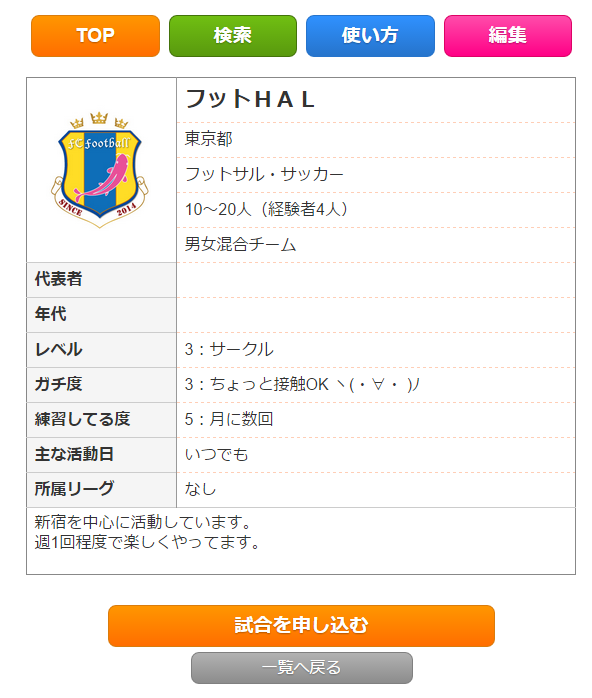
\includegraphics[width=85mm, bb=0 0 800 272]{figures/fl.jpg}
	\caption{footlinkにおける試合相手選択画面 {\itshape http://footlink.net/}}
	\label{footlinkにおける試合相手選択画面}
\end{figure}
\\
\\
選択した後、相手チームから返信がくれば試合を組めることになり、両者で試合の日時、場所を専用取引フォームで進めていくこととなる。
\\ 原則として対戦チーム数は2チームで催され、どちらかがフットサルコートの会員でないとサービスは進行できない。

\subsection{EnjoyFutsal}
EnjoyFutsalはフットボールスマイル株式会社が運営するフットサルチーム同士のマッチングサービスである。メールアドレスで新規登録した後に、画面の図から試合を募集しているチームを選択することで、試合を組むことができる。
\begin{figure}[htbp]
	\centering
	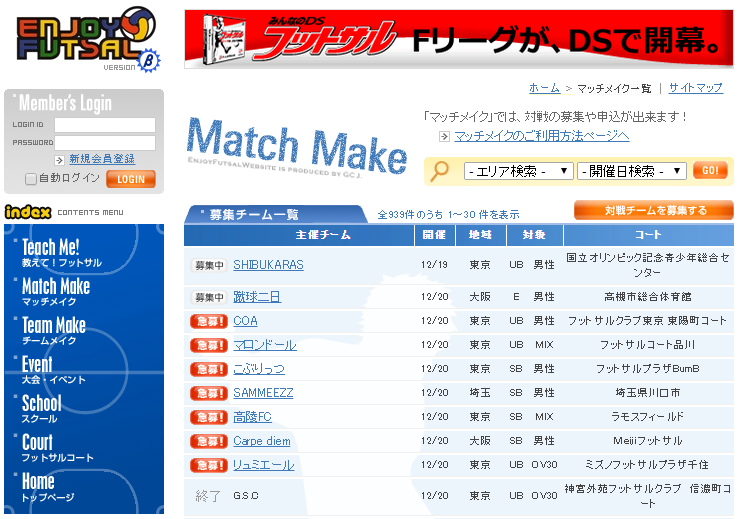
\includegraphics[width=85mm, bb=0 0 800 272]{figures/ef.jpg}
	\caption{EnjoyFutsalにおける試合相手選択画面 {\itshape enjoyfutsal.com}}
	\label{EnjoyFutsalにおける試合相手選択画面}
\end{figure}
\\
\\
\\
\\
特徴としては、3チーム以上のマッチングができる点とチームメイクができる点が、FootLinkと異なる。
\\ 画面にあるように募集チームは男女別、さらにはポジション別にメンバーを募集できる。
\\
\\
\\
\\
\\
\\
\begin{figure}[htbp]
	\centering
	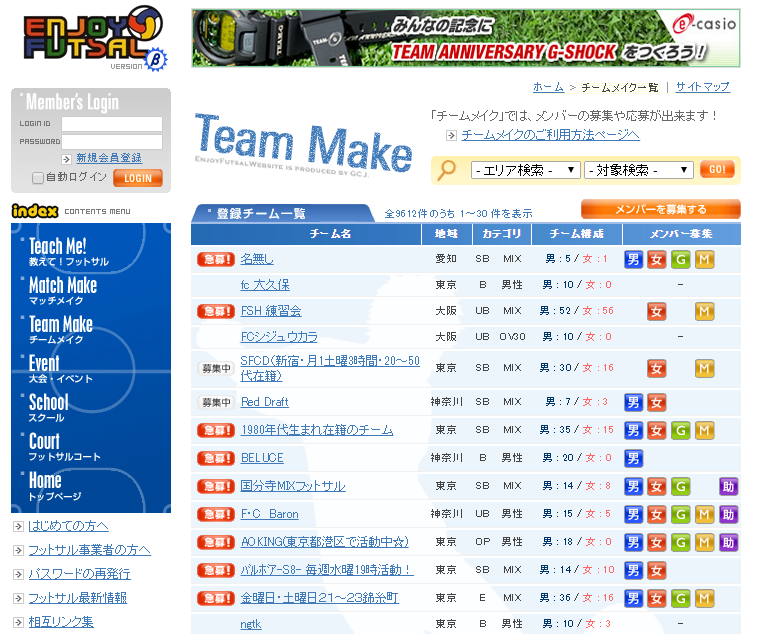
\includegraphics[width=85mm, bb=0 0 800 272]{figures/mm.jpg}
	\caption{footlinkにおける試合相手選択画面 {\itshape enjoyfutsal.com}}
	\label{EnjoyFutsalにおける部員募集画面}
\end{figure}
\section{フラッシュマーケティングの有効性}
フラッシュマーケティングには、クーポンとしての経済的効果と共同購入としての経済学的効果があるとで述べられている。
\subsection{クーポンの経済学的効果}
まずクーポンについての経済学的効果として(玉井、2010)では出稿する店舗側には広告効果、価格差別、スイッチングコスト、リピート効果の4つが述べられている。
本サービスでは、価格とリピート効果に関連し、サービスを構築したのでここでは価格とリピート効果についてどのような経済的効果があるのか述べる。
\subsubsection{価格差別}
クーポン戦略の2つ目の利点は価格差別が行ることである。価格差別には以下3点の特徴がある。 (西岡、2010)
\begin{itemize}
	\item 第1価格差別
	\\財の売り手が、「買い手が支払ってもいい最大の金額」を完全に把握していて、かつ買い手ごとに異なる価格を提示できる。
	\item 第2価格差別
	\\財の売り手は、買い手の特徴や購買意欲によっては異なる価格を提示できないが、財の個数(や品質)と価格の組み合わせを非線形にして提示できる。
	\\具体例としてはガス料金や電気料金といった公共料金、携帯電話の使用料金が挙げられる。
	\item 第3価格差別
	\\財の売り手は、買い手の購買意欲によって異なる価格を提示することはできないが、買い手の特徴(性別、年齢、地域など)によって異なる価格を提示できる。
	\\具体的な例としては,学生割引,女性割引,子供料金,シニアー料金が挙げられる。	
\end{itemize}
Webにおけるクーポンは消費者の登録情報を基に効率よく提供されているので、第3種価格差別が当てはまるので、ここでは第3種価格差別の話を進めていく。
\subsubsection{リピート効果}
\subsection{共同購入の経済学的効果}
(Evan Miller,2012) によると図で多数の購買者が集まって低価格で買うことにコミットすれば従来にない需要と供給のマッチングポイントが生まれ、買い手と売り手にっとって新しい有効性があると論じている。
\begin{figure}[htbp]
	\centering
	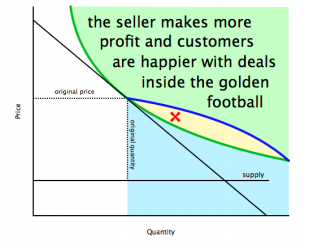
\includegraphics[width=85mm, bb=0 0 200 272]{figures/nush.jpg}
	\caption{フラッシュマーケティングにおける価格均衡点 {\itshape http://www.evanmiller.org/golden-football.html}}
	\label{フラッシュマーケティングにおける価格均衡点}
\end{figure}

\chapter{ビジネスモデル}
\label{intro}

%\makeendnotes  %フットノートをすべて章末に移動するスクリプトです。使用しない場合はコメントアウトしてください。

\section{Liven Up初期ビジネスモデル}
\subsection{現状の課題分析}

本章では、フットサルのマッチングサイトを構築するにあたり現状の課題をフットサルコートオーナーと消費者 (プレイヤー) の観点から分析する。まずフットサルコートのオーナーの観点からみて課題となっているのが集金システムである。現状の集金システムでは消費者 (プレイヤー) から先払いで集金できないため、当日キャンセルによる収益の損失リスクを軽減できていない。
先にも述べたが先払い制を採用してしまうと大会が開催されなくなかった場合、一度集金した料金の返金や集金管理から生じるクレームにつながる。そのため、コート自身による大会運営では先払いシステムを採用できていないのが現状である。
\\ 次に消費者の観点からみて課題となっているのが、自チームだけで練習を行えないメンバー数のチームは、通常価格のコートはもちろん例え格安のフットサルコートを買えないことである。言わずもがな自分たちだけでは練習はできないので、フットサルコートの年間会員になることもできない。これはフットサルコートからしても大きな損失を被っている。メンバーの少ないチームは、フットサルコートが主催する大会に出る以外フットサルをするを機会がない。
\\ この問題を解決するために重要なのは、コートの代わりに集金するシステムとチーム同士をマッチングさせるプラットフォームを持つことである。
る。

\subsection{初期ビジネスモデルの構築}
筆者が所属する慶應義塾大学大学院メディアデザイン研究科杉浦一徳研究室GCMTにおける取組として「Liven Up」プロジェクトを構想した。本プロジェクトはコートの集金損失リスクを避け、立地条件が悪く普段集客しにくい時間帯を割安で貸し出すプラットフォームの開発を目的としている。

【本サービスプラットフォーム内での販売対象コート】
以下、条件を満たすコート
\\・時間帯  :二週間前時点で埋まっていない時間帯
\\・立地   : 駅から徒歩10分以上20分以内
\\・運営形態: フランチャイズ運営ではなく自営運営のフットサルコート

上記のようなコートを対象に、立地条件が悪く利用者が使わない時間帯のコートを「Liven Up」上で公開し、フットサルチームとコートをマッチングさせる仕組みである。

協力コート:FUNフットサルコート



\begin{figure}[htbp]
	\centering
	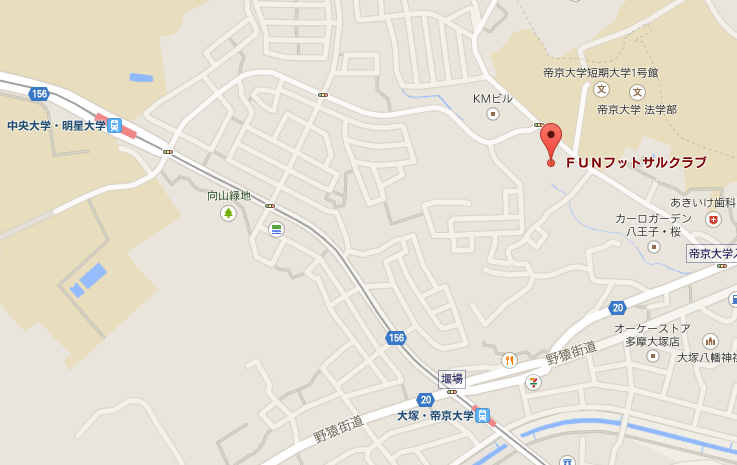
\includegraphics[width=85mm, bb=0 0 600 400]{figures/fun.jpg}
	\caption{Funフットサルクラブ所在地 {\itshape Google Map}}
	\label{Funフットサルクラブ所在地}
\end{figure}




【ビジネスフロー】
\\
・コートのLiven Up上への空きコート情報の掲載は無料
\\・ユーザーはLiven Up上で1試合5000円のチケットを事前に支払い、曜日を指定した後フットサルの試合に参加
\\・Liven Upが集金した料金の6割をコートへ支払う
\\
上記条件に基づくビジネスフローより、フットサルコートはコートのアイドリングタイムを減らしつつ、レンタルコートという仕組みで儲けることができる。同時に、集金する手間や大会への審判、タイムキーパーを用意する手間を省いた仕組みの構築を実現した。
また、コートの利用者は従来型のレンタルコートが提供するサービスの価格と比べ、約半分の価格水準でコートを利用することが可能となり、対戦相手を容易に見つけることをサポートすることを仕組化した。

\begin{figure}[htbp]
	\centering
	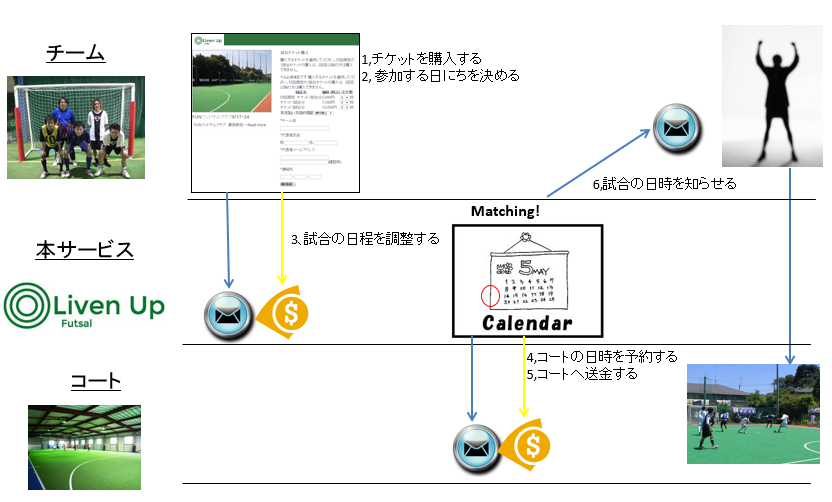
\includegraphics[width=85mm, bb=0 0 500 400]{figures/bm.jpg}
	\caption{初期ビジネスモデル {\itshape 初期ビジネスモデル}}
	\label{初期ビジネスモデル}
\end{figure}




\section{初期ビジネスモデルの検証}
 サービスの運営にあたり、前節で紹介したビジネスモデルについて、2014年4月から6月にかけて2試合をマッチングした。
 参加者の条件は下記の通りにした。
 \\ 「LivenUp」の各ステークホルダーにヒアリングした結果は以下の通りである。
 \par
 【サービスのコンセプトについて】
 \\ ・人件費をかけずにコートを使ってもらえるので、非常に有益なツールだと思う。(コートオーナーN氏)
 \\・人数の少ないチームにとって、大会に比べ安価かつ簡単にチームを見つけることができるのはありがたい。 (フットサル参加者S氏)
 \par
 \\\textbf{【サービスの料金体系について】}
 \\・ちょうどいい (社会人フットサルチームA氏)
 \\・他チームを紹介したら、割引がほしい。 (学生フットサルチームM氏)
 \par
 \\\textbf{【サービスの内容 (試合時間や試合本数、運営について) 】}
\\ ・実際にチームを探す手間や当日に来ないリスクがないので安心して使える。 (学生フットサルチームS氏)
 \\・審判は自分たちでやらなくても、タイムキーパーさえいれば運営は成立する。 (社会人フットサルチームA氏)
 \\・受付にいったらどこのコートでやるのか等々、指示がほしい。 (学生フットサルチームT氏)
 \\・当日の運営をどのチームが仕切るのかわからない。(学生フットサルチームM氏)
 \\・試合当日に支払いする手間が省けたので、気軽に行ける。(学生フットサルチームK氏)
 \\・当日の欠席もなく、銀行振り込みなので、安心できる。(フットサルコートオーナーN氏)
 \par
 \\\textbf{【マッチングの仕組みについて】}
\\ ・レベルの強さはあまり問わないが、最低限どういうチームが来るのか知りたい。 (社会人フットサルチームA氏)
 \\・体力別、学生別等々でセグメントを分けてマッチングしてほしい。(社会人フットサルチームI氏)


\subsection{サービスの修正}
以下サービス内容に修正を加えた。

【試合当日の運営について】
上記で観察されたように、各チームコートが到着した段階では、どこのチームが試合の運営をするのか、もしくはコート側が運営を始めるのかサイト上の情報だけでは、十分に伝わっていなかったと考えられる。この問題を解消するため、試合の前日のリマインダーメールに当日の運営内容を記載したメールを各チームに送付した。またボールの片づけや開始の準備をするチームをランダムで選び指定し、メールで伝えた。









%\input{approach.tex}
\chapter{サービス設計}

\section{サービス概要}
前節で述べたビジネスモデルをもとに2013年9月下旬からwordpressを活用し、サービスの開発を開始した。開発と並行し、株式会社手嶋屋に協賛企業としてプロジェクトに参加して頂き、彼らのサービスであるオリジナルのソーシャルネットワークを作成できるpne.jpとクレジットカードを使ってクラブ活動の毎月の集金を自動化することができるpne.clubをプロジェクトに無性に提供して頂いた。

【協賛企業】

企業名:株式会社手嶋屋
サイト:http://www.tejimaya.com/
協賛内容:ソーシャルネットワーク作成ツールpne.jpとクラブ集金ツールpne.clubの無償提供
\section{サービスコンセプト}
サービスのローンチにあたり、Liven Upのサービスコンセプトを「手軽に格安でフットサルの試合を組めるプラットフォーム」とした。本サービスで試合をマッチングすることで、フットサルコートのアイドリングタイムを手間をかけずに有効に活用できることを目標とした。

\begin{itemize}
	\item フットサルプレイヤーは、簡単にフットサルの試合相手を見つけることができ、格安で参加できる。
	\item コートは効率的に空きコートを埋めることができる
	\item 参加者のみで試合を運営できる
\end{itemize}
\section{サイトデザイン}
\subsection{トップページ}
トップページでは図で示した通り、一目で各フットサルコートの情報を訴えかけられるように各フットサルコートを並べて、利用者の立地条件が一番コートを選んでもらえるようにした。予約のタブを押すと利用者が予約したい日時を決めるページに飛ぶ。
\\
\\
\\
\\
\\
\begin{figure}[htbp]
	\centering
	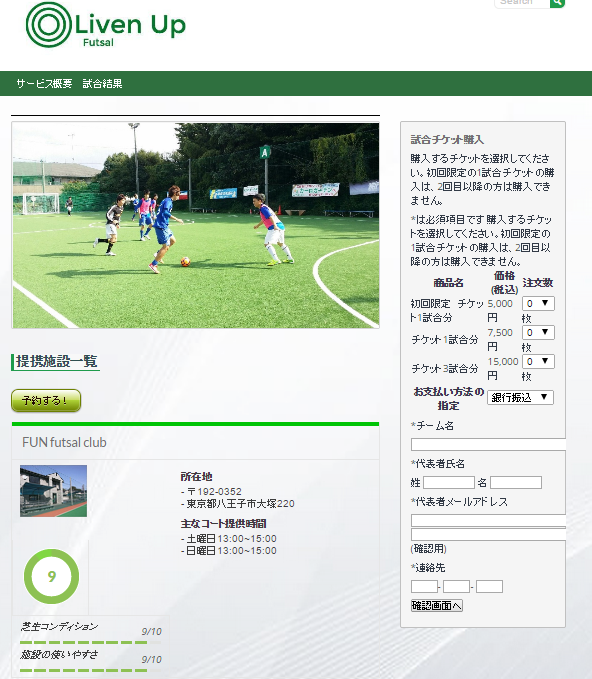
\includegraphics[width=85mm, bb=10 0 500 300]{figures/top.jpg}
	\caption{施設情報 {\itshape Google Map}}
	\label{施設情報}
\end{figure}

\newpage

\subsection{チケット購入ページ}
画面右には本サイト内で購入できるチケットの購入ページを配置した。初回のみ5000円で購入できるが、2回目以降は一回7500円、3試合分のチケットをまとめて購入すると15000円で購入できる。まとめて購入してもらうことにより多くのチームに試合に参加できる選択肢を持たせる価格設定にした。
\\
\\
\\
\\
\\
\\
\begin{figure}[htbp]
	\centering
	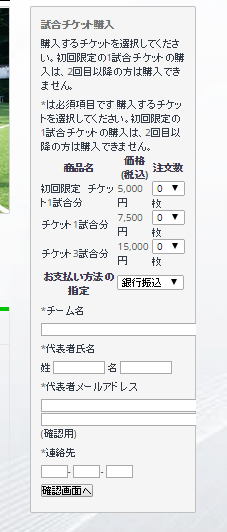
\includegraphics[width=85mm, bb=30 0 300 300]{figures/buy.jpg}
	\caption{購入画面 {\itshape Google Map}}
	\label{購入画面}
\end{figure}
\newpage


\subsection{フットサルコート情報}
フットサルコートの情報を所在地やコートの主な使用できる時間帯、各指標を示した。また気に入ったらワンタッチで予約ができるように予約タブを配置した。
\ 次のページで、予約可能の日時一覧が出てきて、新たに予約できる都合の良い日時にエントリーできるようになっている。
\\
\\
\\
\\
\\
\begin{figure}[htbp]
	\centering
	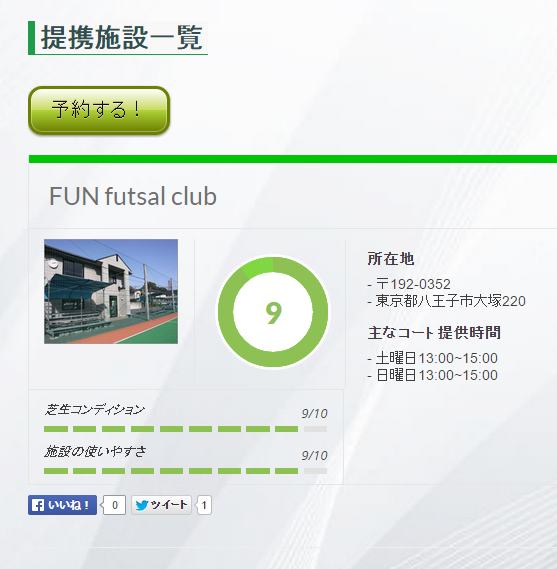
\includegraphics[width=85mm, bb=0 0 300 300]{figures/book.jpg}
	\caption{施設情報 {\itshape Google Map}}
	\label{施設情報}
\end{figure}
\newpage
\begin{figure}[htbp]
	\centering
	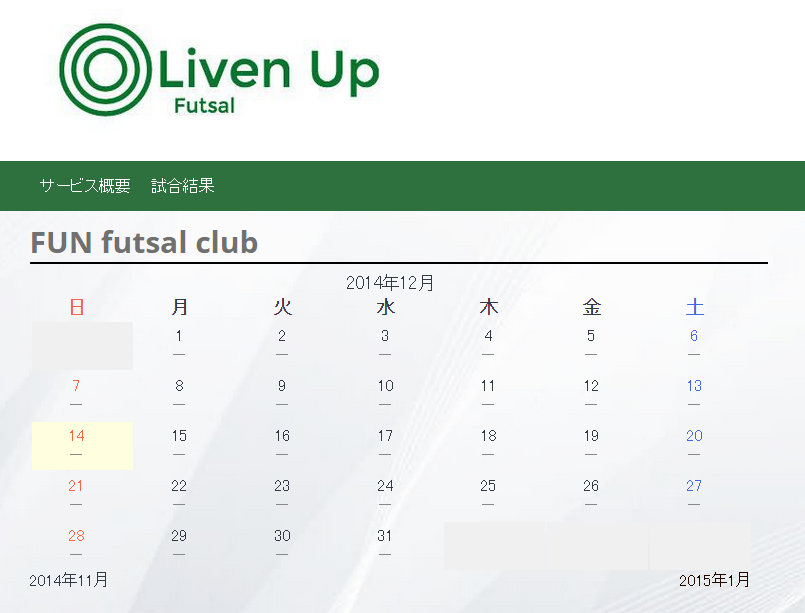
\includegraphics[width=85mm, bb=0 0 400 300]{figures/date.jpg}
	\caption{予約画面 {\itshape Google Map}}
	\label{予約画面}
\end{figure}
\newpage



\section{ステークホルダー別サービス利用フロー}
本節では本サービスのステークホルダーのサービス利用フローについて説明する。

\subsection{フットサルコートの利用フロー}
フットサルコートのオーナーは1章のインタビューでもあった通り、できるだけにクーポン出稿に際した文言や手間を省いた。
\\ 先にも紹介した通り、各フットサルコートのページは固定であり、フットサルコートのオーナーは主に本サイトのメールアドレスにコートが予約が入っていない時間帯を送るだけである。
\\ 本サイトのスタッフでフットサルコートの予約できる時間帯を随時更新していき、予約が埋まり次第、コートに電話をし、コート抑え、翌日営業以内に送金をする仕組みである。


\subsection{プレイヤーの利用フロー}
 購入ページからチケットを購入したのちに、各コートの予約ページから都合のよい時間帯を選び予約する。
 \\ 予約をしてから3日ごとに利用者に報告するようしている。成立する場合でも4日前までには連絡する仕組みである。
\chapter{サービス運営}

\section{運営概要}
2014年8月に下旬に運営を開始してから、約3ヶ月のサービスの運営についての振り返りを実施した。当該期間に本サービスを用いて3試合がマッチングされ、79名に使用してもらった。
当期間の試合は下記3点の項目を検証するため、チームの抽出条件を下記のように設定した。
\begin{itemize}
	\item チーム数:9チーム (お互い試合をしたことがないチーム同士)
	\item 参加者の性別:男性のみ
	\item 職業:大学生:社会人
	\item 年齢層:20-25歳
\end{itemize}



当期間で下記3点の仮説を検証した。
\begin{itemize}
	\item[$H1$] 自分たちだけで試合を運営できるのか
	\item[$H2$] 本サービススタッフがコートに行かなくても試合を運営できるのか
	\item[$H3$] どれくらいのチーム数と試合時間が適切か
\end{itemize}






\section{2014年10月までの運営振り返り}

2014年8月に下旬に運営を開始してから、9月3日までの約1ヶ月のサービスの運営についての振り返りを実施した。当該期間に本サービスを用いて3試合がマッチングされ、33名に使用してもらった。
\\
\\
\\\textbf{【ファーストテスト( 8月30日)】}
\\1度目のテストを行い、検証項目である「自分たちでだけで試合が運営できるのか」という項目を検証した。
3チームが参加し、7分の試合を2時間行った。各参加者の詳細は表のとおりである。
\\ 事前に参加者には参加者のでタイムキーパーと審判を決めて回すように伝えておいた。

\begin{table}[htb]
	\begin{center}
		\caption{ファーストテスト (2014年8月30日)}
		\begin{tabular}{|l|c|r||r|} \hline
			チーム人数 & 活動頻度 & 値段についての感想 & 試合時間についての感想 \\ \hline \hline
			5人(社会人のみ) & 月一度程度 & ちょうどよい & 長く感じた \\
			7人(学生のみ) & 週2回 & 安い & ちょうどよい \\
			7人(学生3人) & 週2回 & ちょうどよい & ちょうどよい \\ \hline
		\end{tabular}
		\label{tab:price}
	\end{center}
\end{table}

タイムキーパーや審判がいなくても運営は成功したが、当日コートに到着してもどこのコートでやるのかわからなくて試合の時間が遅れてしまった。理由は2点ある。1点目はどこのコートで行われるかわからなかったためである。よって事前に送るメールに一度受付に行って当日のコートを確認してもらう必要がある。また当日の準備するチームと片づけをするチームが明確でなかったため、コートの準備に遅れが生じた。コートのビブスやボールも片づけられることがなかった。
\\
\\
\\\textbf{【セカンドテスト( 9月21日)】}
\\
\\
2度目のテストを行い、検証項目である「本サービスのスタッフが当日行かなくても運営できるか」という項目を検証した。
2チームが参加し、7分の試合を2時間行った。各参加者の詳細は表のとおりである。
\\ 受付で当日の試合が行われるコートと準備と片づけについて指示した。

\begin{table}[htb]
	\begin{center}
		\caption{セカンドテスト (2014年9月21日)}
		\begin{tabular}{|l|c|r||r|} \hline
			チーム人数 & 活動頻度 & 値段についての感想 & 試合時間についての感想 \\ \hline \hline
			13人(学生のみ) & 週3回 & ちょうどよい & ちょうどよい \\
			15人(学生のみ) & 週2回 & ちょうどよい & ちょうどよい \\ \hline
		\end{tabular}
		\label{tab:price}
	\end{center}
\end{table}
事前に送ったメールのマニュアル通り運営したため
後日、参加者にインタビューをしたところいつものように試合ができたという意見を貰った。
\\コートの片づけもされていたので、コート側の余計な労働はなかった。
\\
\\\textbf{【ファーストテスト( 9月27日)】}
4チームで7分の試合を2時間行った。チーム数を増やすことによって試合への満足度に変化が見られるのか調べた。

\begin{table}[htb]
	\begin{center}
		\caption{ファーストテスト (2014年9月27日)}
		\begin{tabular}{|l|c|r||r|} \hline
			チーム人数 & 活動頻度 & 値段についての感想 & 試合時間についての感想 \\ \hline \hline
			5人(社会人のみ) & 月一度程度 & ちょうどよい & 長く感じた \\
			5人(社会人のみ) & 月二回程度 & ちょうどよい & 長く感じた \\
			14人(学生のみ) & 週2回 & 安い & ちょうどよい \\
			8人(学生のみ) & 週2回 & 安い & ちょうどよい \\ \hline
		\end{tabular}
		\label{tab:price}
	\end{center}
\end{table}

待ち時間が長くなるので、7分の試合時間を5分程度にして、より多くの試合を回すことが重要であった。
2014年8月30日から1ヶ月の運営期間をもとに考察したLivenUpの成果と課題は下記のとおりである。

\subsection{【成果】}
・コートのアイドリングの時間を格安でフットサルチームが共有することでコートのアイドリングタイムで新たに稼ぐ手段ができ、需要があることを確認できた
\\
・事前のメールを送り、準備や片づけを指示したことで運営はスムーズにいった
\\
・最適なゲーム時間は3チームで7分がちょうどよかった
\subsection{【課題】}
・本サービス内のクーポンをすべて使用してしまった後に引き続き継続してもらうにはどうすればいいか。最初にクーポンを3枚購入したチームは3チームいたが、継続で買ってもらう際のクーポンの枚数はどのチームも1枚だった。
\\・本サービスにTwitterやFacebookを通して、新たなに参加したチームはいなかった。新規にユーザーを獲得する方法を模索する必要がある。
\\・アマチュアだけが参加することで、レベル感に不安を感じるユーザーはいなかったが、予めどのような属性 (学生、週の練習回数)のチームが来るなど事前に知らせることで不安を軽減する必要がある。
\\・本サービスを決済する際に、事前にチームメイトから集金でき、そのままシームレスに本サービスの決済を済ませることができればより決済周りの煩雑性は解消される。





\section{機能改善}
上記にもあるようにチーム内の集金のあり方を変えた。具体的には株式会社手嶋屋のpne.clubを用いり、クラブ内のメンバーからの集金を可能にすることで、代表者が一括で試合代金を負担することがないシステムを採用した。


\chapter{サービスの評価}
\section{調査概要}
本章では、2014年8月下旬から運営を開始して以降のサービスの運営内容を計測し、今後に向けての成果や課題を考察する。
\\ 定性調査として、本サービスの対象となるフットサルのコートのオーナー、プレイヤーへのインタビュー調査を実施することで、より客観的な調査結果を得ることができるように努めた。
またコートは本サービスで得た収入をどのような経営形態を変化させたのかを考察する。
\\ 本サービスを利用して頂いたコートのオーナーおよびフットサルチームのプレイヤーに本サービスの概要及び「購入ページ」、「予約ページ」、「コートの状況」といった各ページについてインタビュー調査を行った。
\section{調査結果:フットサルプレイヤー}
【サービス全体について】
\\プレイヤーから格安で試合ができ、試合相手を探す手間を省くことができたことが高い評価を得た。コートからは集金機能を本サービスが担うことで、集金する手間が省けるだけではなく、利益の損失するリスクを軽減できたことが評価された。
\\しかし、新サービス故の信頼性を指摘された。画面上部にある利用規約や運営者の情報を見やすい部分に設置することを指摘された
\\【購入ページについて】
\\会員制のページにしてほしい。一度、購入したら二度目以降はメールアドレスの記入等々を省いてほしい
\\【予約ページについて】
・カレンダー形式に表示するより、開催予定の日時だけを表示してほしい
【今後、本サービスに望むこと】
\\今後、本サービスに望まれていることは、下記3点である。
\\・会員制登録ページを作ってほしい
\\・同じ地域で運営する場合、最低3つは候補地があったほうがいいと指摘された
\\・淡々と試合をするだけでは、面白みに欠けるという意見出た。今後、モチベーションを上げるための景品などを用意したほうがいいという意見が出た




\section{調査結果:フットサルコートオーナー}
【サービス全体について】
\\コートからは集金機能を本サービスが担うことで、集金する利益の損失するリスクを軽減できたことと日程をエクセルシートで送付するだけで手間がないことが評価された。

【サービスによる収支について】
\\本サービスで一回分の試合をマッチングさせることで、コートはアルバイト1人分の日給に値する収入得ることが分かった。今後、これを週5日送客することで、アルバイト二人分の人件費に充てることができるとわかった。

【今後、本サービスに望むこと】
\\本サービスを用いて、フットサルコートの会員になるチームがなかった。今後、コートに会員登録してもらえるようにチームの人数を増やす仕組み、本サービスだけでコートに送客ができることを期待されている。言い換えるのであれば、サイト内のPV数を増やすことが望まれている。


\section{考察}
本節にてここまで記述してきたインタビュー調査についての結果について分析を実施する。
\\サービス利用者であるフットサルプレイヤーからは、価格面、サービスを通じて手軽にマッチングできる点から概ね高い評価を得ることができた。
今後、新規に利用者を獲得するには、紹介制を活用するだけではなく土地や年齢層にリーチできる広告媒体を選択し活用していくことが重要であると考える。
\\またサービス全体の規模としてはまだ東京都八王子での運営に留まっており、サービスの規模は小さくビジネスとして成立しているとは言い難い。
\\ 今後サービスを拡大していくには上記の利用者の母数を増やし、利用者のコメントを本サイト内で掲載し信頼を高めていくことに加えて、コートに定期的に送客できる仕組みを作ることが重要である。




\chapter{結論と今後の課題}
\label{intro}
\section{運営総括}
2013年10月に本プロジェクトを構想して以降、株式会社手嶋屋の協力のもと、2014年8月にフットサルマッチングサイトであるLivenupをローンチすることができた。特に10月は月に3試合が組まれ、紹介を通じ、若干ではあるが新規会員が増えた。2013年12月までに8試合を催すことできた。今後は、徐々に本サービスの認知度を上げ、新規利用者の自然流入を図っていく必要がある。実際に2015年2月からは提携コートを増やし、店頭に本サービスのチラシを配布する予定である。
\\ サービスの運営を通じて「フットサルチームのマッチング」および「フットサルチームのアイドリングタイムの有効活用」を目的に、フットサルチームに格安でコートを提供しフットサルコートのアイドリングタイムを削減に成功した。これまでフラッシュマーケティングサイトがレジャーカテゴリーにおいてできていなかったシステムを構築し、新たに利用者へのニーズ喚起させ、満たしたと言える。ただ一方、また運営上の課題も多々あげられるので、次節以降で述べる。
\section{運営成果}
本サービスはインタビュー調査をもとに、従来のフラッシュマーケティングの問題点を洗い出し、サービスの仕組みを構築した。複数チームで共有することでコートのアイドリングタイムを活用できることがわかった。
\\ 本サービスが集金し、先払いを利用者に強いることで、従来フットサルコートが問題視していた当日のキャンセルのリスクは軽減され、アイドリングタイムで収入を得ることができた。
\\ この仕組みはフラッシュマーケティングが対象としているスポーツ施設に応用できる可能性がある。具体的にはテニスコートやゴルフ場など登録制のクラブで本サービスの仕組みを応用できると考える。
\section{今後に向けた課題}
運営上の課題は、現状では提供できるフットサルコートが少ないことと利用者への認知度が低いことである。フットサルコートを
今後は利用できる提携フットサルコートを増やした上で、利用者を徐々に増やしていく必要がある。
\section{サービス改善}
今後、本サービスを運営するにあたりに以下の2点が挙げられる。
\\\textbf{・集金システムの改善}
\\ チーム内での集金を試合当日に行うのではなく、本サービスで決済する前にチーム内で集金できるシステムがあれ代表者の決済の負担が軽減できると考え、株式会社手嶋屋のpne.clubを用いて、システムを採用してくれるチームを現在募集中である。
\\
\\\textbf{・コートごとに手数料を変える}
\\次にコートへの支払い金額についてである。Funフットサルクラブはフットサルスクールをメインの収入源にしていたため、自ら新規顧客を集約する力がなかったので、Livenupからの紹介手数料の意味合いを込めて、集金代金の50%を徴収していた。ただ東京都郊外のフットサル場には個人で参加し、即席チームで戦う個人フットサルで収入を得ているフットサルコートもある。個人の情報は多く保持しているが、前払い制ではないため当日にキャンセルされる可能もあるため本サービスの仕組みは有効である。このようにコートによって収入源が違うので、コートの経営形態に合わせた手数料を設定していく必要がると考える。



%\input{futurework.tex}
%\input{conclusion.tex}
%
% 謝辞
%
\acknowledgements

本研究の指導教員であり、
幅広い知見から的確な指導と暖かい励ましやご指摘をしていただきました慶應義塾大学大学院
メディアデザイン研究科の杉浦一徳教授に心から感謝いたします。

研究の方向性について様々な助言や指導をいただきました慶應義塾大学大学院 メディアデザイン研究科の岸博幸教授に心から感謝いたします。

研究指導や論文執筆など数多くの助言を賜りました慶應義塾大学大学院 メディアデザイン研究科の稲見昌彦教授に心から感謝いたします。
%
% 参考文献
% ここでは \reference を使って、自分でリストを作るか、BibTeX を使って
% リストをつくって下さい。この例では BibTeX を作るような形式になっ昌彦
% ます。
%
\newpage
\reference

%\nocite{*} %bibtexにリストされている、すべての文献を表示させたい場合は使用する。(本文中で引用されたものだけ使用する場合はこのまま)

%%%%%%%%%%%%%%%%%%%%%%
%Style of Bibliography
%%%%%%%%%%%%%%%%%%%%%%

%Chicago Style that can also use Japanese citations
%\bibliographystyle{jecon_edit}

%Numbering Style (General Science Format)
%\bibliographystyle{abbrv}

%ACM SIGCHI Style
\bibliographystyle{acm-sigchi}

%%%%%%%%%%%%%%%%%%%%%%%

\bibliography{document}
\begin{thebibliography}{9}
	\bibitem{yauchi,2012} C. Harris and M. Stephens,
	``A combined corner and edge detector, '' Proc. 4th Alvey Vision Conf.,
	pp.147-151, Manchester, U.K., Aug. 1988.
	\bibitem{susan} S. M. Smith and J. M. Brady,
	``SUSAN|A new approach to low level image processing,'' Int. J. Comput.
	Vis., vol.23, no.1, pp.45-78, May 1997.
\end{thebibliography}
%
% 付録
%
%\appendix
%\section{障害検知設定ファイルの例}
%障害検知の設定ファイルを以下に示す。
\begin{verbatimtab}
<config>
<system>
<class>DefaultCompareClass</class>
</system>
<evaluate>
<compare_single_observation_point>
<function method="compareMax" recital="Temperature maximum threshold value"
type="Temperature"> <argument class="double">40.8</argument>
</function>
<function method="compareMin" recital="Temperature minimum threshold value"
type="Temperature"> <argument class="double">-41.0</argument>
</function>

<function method="compareChange" recital="Temperature change amount error"
type="Temperature"> <argument class="double">17.0</argument>
<argument class="int">1</argument>
</function>

<function method="compareConstant" recital="Temperature constant error"
type="Temperature"> <argument class="int">1</argument>
</function>
</compare_single_observation_point>

<compare_neighbor>
<function method="compareNeighbor" recital="Temperature neibor error"
type="Temperature"> <argument class="double">2.0</argument>
</function>
</compare_neighbor>

<compare_wide_area>
<function method="compareWide" recital="RainFall wide area error"
type="RainFall"> <argument class="double">10.0</argument>
</function>
</compare_wide_area>
</evaluate>
</config>
\end{verbatimtab}
%\begin{figure}[t]
%\begin{center}
%\includegraphics[width=120mm, height=100mm]{./figure/config.eps}
%\caption{障害検知設定ファイルの例}
%\label{appendix1}
%\end{center}
%\end{figure}

\end{document}
